%%%%%%%%%%%%%%%%%%%%%%%%%%%%%%%%%%%%%%%%%%%%%%%%%%%%%%%%%%%%%%%%%%%%%
%%%
%%% Set these variables appropriately
%%%
\newcommand{\AUTHORS}{YOUR NAME HERE}
\newcommand{\TITLE}{PAPER TITLE HERE}
\newcommand{\KEYWORDS}{}
\newcommand{\CONFERENCE}{}
\newcommand{\PAGENUMBERS}{yes}       % "yes" or "no"
\newcommand{\TOAPPEAR}{no}
%%%
%%%
%%%%%%%%%%%%%%%%%%%%%%%%%%%%%%%%%%%%%%%%%%%%%%%%%%%%%%%%%%%%%%%%%%%%%

%%%% Setup the document/page
\documentclass[pdftex,twoside,twocolumn,11pt,letterpaper]{article}
\usepackage{ifthen}

\ifthenelse{\equal{\PAGENUMBERS}{yes}}{%
\usepackage[nohead,
            left=1in,right=1in,top=1in,
            footskip=0.5in,bottom=0.75in     % Room for page numbers
            ]{geometry}
}{%
\usepackage[noheadfoot,columnsep=0.2in,
            margin=1in,centering,truedimen]{geometry}
}

\usepackage{fancyhdr}
\usepackage[numbers,sort]{natbib}
\usepackage{xspace}
\usepackage{booktabs}
\usepackage{subfigure}
\usepackage[T1]{fontenc}
\usepackage{textcomp}
\usepackage{mathptmx}   % Times + Times-like math symbols
\usepackage{courier}
\usepackage[scaled=0.92]{helvet}

\usepackage{color}
\usepackage[pdftex]{graphicx}
\ifthenelse{\isundefined{\wantBW}}{%
  \usepackage[colorlinks]{hyperref}%        % for online version
}{%
  \usepackage[pdfborder={0 0 0}]{hyperref}% % for paper (B&W) version
}
\newcommand{\URL}[1]{\url{#1}}

%%%%% Setup for PDF
\hypersetup{%
pdfauthor = {\AUTHORS},
pdftitle = {\TITLE},
pdfsubject = {\CONFERENCE},
pdfkeywords = {\KEYWORDS},
bookmarksopen = {true}
}

%\setlength{\parindent}{0pt}
%\setlength{\parskip}{0pt}
\renewcommand{\headrulewidth}{0pt}
\newcommand{\Paragraph}[1]{\vspace{-2ex}\paragraph{#1.}}
\setlength{\topmargin}{-.15in}

\ifthenelse{\equal{\PAGENUMBERS}{yes}}{%
  \pagestyle{plain}
}{%
  \pagestyle{empty}
}

\makeatletter\long\def\@makecaption#1#2{
   \vskip 10pt
   \setbox\@tempboxa\hbox{\textsf{#1: #2}}
   \ifdim \wd\@tempboxa >\hsize % IF longer than one line:
       \textsf{#1: #2}\par      % THEN set as ordinary paragraph.
     \else                      % ELSE  center.
       \hbox to\hsize{\hfil\box\@tempboxa\hfil}
   \fi}
\makeatother

\clubpenalty=10000  % Don't allow orphans
\widowpenalty=10000 % Don't allow widows

\title{\textbf{\TITLE}}
\author{\AUTHORS}
\date{}

% Compact itemize and enumerate.  Note that they use the same counters and
% symbols as the usual itemize and enumerate environments.
\def\compactify{\itemsep=0pt \topsep=0pt \partopsep=0pt \parsep=0pt}
\let\latexusecounter=\usecounter
\newenvironment{CompactItemize}
  {\def\usecounter{\compactify\latexusecounter}
   \begin{itemize}}
  {\end{itemize}\let\usecounter=\latexusecounter}
\newenvironment{CompactEnumerate}
  {\def\usecounter{\compactify\latexusecounter}
   \begin{enumerate}}
  {\end{enumerate}\let\usecounter=\latexusecounter}

\newcommand{\comment}[1]{\textcolor{red}{#1}}
\newcommand{\ignore}[1]{}

\newcommand{\xc}[1]{\mbox{\textit{#1}}}
\newcommand{\la}{\leftarrow}
\newcommand{\ra}{\rightarrow}
\newcommand{\somespace}{\hspace{0.1cm}}

\def\discretionaryslash{\discretionary{/}{}{/}}
\def\discretionarydot{\discretionary{.}{}{.}}
\def\discretionarycolon{\discretionary{:}{}{:}}
{\catcode`\/\active
\catcode`\.\active
\catcode`\:\active
\gdef\URLprepare{\catcode`\/\active\let/\discretionaryslash
                 \catcode`\.\active\let.\discretionarydot
                 \catcode`\:\active\let:\discretionarycolon
        \def~{\char`\~}}}%
\def\URL{\bgroup\URLprepare\realURL}%
\def\realURL#1{\tt #1\egroup}%

\newcommand{\eg}{{\em e.g.}, }
\newcommand{\ie}{{\em i.e.}, }
\newcommand{\etal}{{\em et al.\ }}

\def\check{\stackrel{{\scriptscriptstyle ?}}{=}}

\begin{document}
\maketitle

% -*-LaTeX-*-
% $Id: abstract.tex 70 2007-01-30 21:59:16Z nicolosi $

\begin{abstract}
High performance applications such as {\emph{in-memory key-value stores, web server accelerators, etc.}} require large amounts of memory. However, these applications have heavy tailed memory access footprints. In this paper, we present the design and implementation of Tracer: a tool that allows developers to trace memory accesses at object level granularity. The design philosophy of Tracer is to assist applications in identifying {\emph{entities}} (such as C level {\emph{structures}}) which get heavily accessed. Tracer accomplishes this with negligible intrusion into the application code, allowing for easy integration with existing projects. We evaluated a prototype implementation of Tracer and observed only reasonable overheads of $28\%$ and $40\%$ over non-modified C code for creation and read heavy workloads, respectively. As compared to a page protection mechanism, Tracer improves the average performance by $12\%$ and $6.28\%$ for read and update heavy workloads, repectively. 
\end{abstract}

   
\section{Introduction} 
\label{sec:intro}
\paragraph{}
For traditional C based high-end applications, memory tracing is a difficult problem to resolve since most of the accesses to memory occur through hardware. Software based techniques such as those used by {\emph{Valgrind's memcheck \cite{nethercote2007valgrind}} and {\emph{gdb's ptrace}} \cite{gdb} rely on memory protection mechanisms which introduce heavy overheads. Therefore, these techniques cannot be effectively used for monitoring high performance applications. This work presents the design, implementation and evaluation of Tracer, a code based instrumentation system coupled with memory monitoring techniques which enables applications to transparently obtain information on their memory footprints with low overhead. 

\paragraph{Design philosophy}
Tracer provides APIs for efficient tracking of object-level memory accesses. Previous works on object caching make use of memory protection mechanisms, resulting in page faults on object accesses and high virtual memory space utilization. We aim to minimize overheads while providing useful information to the application programmer. This information can assist application developers in enhancing application performance by compact placement of "hot" objects. This would reduce access latencies and result in better memory usage. Overall, the philosophy underlying the design of Tracer's architecture is outlined as follows:
\begin{enumerate}
\item The interception mechanism must be transparent to the application developer.
\item The interceptor and the memory monitoring libraries must be easily pluggable into a standard C application.
\item The overall overheads must be reasonable compared to the performance of a vanilla C application (an uninstrumented C application).
\item The design must be system independent (i.e. independent of POSIX system calls such as protection mechanisms and reliance on system dependent hardware or architecture).
\end{enumerate}

\paragraph{}
This work presents the design of Tracer. Tracer provides a C pre-processing tool called the {\emph{interceptor}} and a set of APIs (bundled with the standard GNU C library) for monitoring and providing the overall memory access footprint at an object-level granularity to C application developers. Tracer achieves all the objectives outlined above. The interceptor uses preprocessing using standard code parsing and injects {\emph{"memlets" (memory access calls)}} into the C program, thus making the design transparent to the application developer and easily pluggable into a standard C applications. The monitoring library is implemented as a part of the standard GNU C library.  The solution does not depend on hardware or require additional hardware and is therefore independent of the platform used. Our implementation on binary tree micro benchmarks reports an overhead between roughly $20\%$ and $40\%$ for create and read workloads, repectively. We therefore believe that Tracer is a useful and efficient software solution which could assist application development by providing better memory monitoring.


\paragraph{}
The paper is organized as follows: Section \ref{sec:motivation} outlines the motivation underlying our work.  Section \ref{sec:design} describes the design of Tracer. Section \ref{sec:eval} describes the microbenchmark study and a discussion of results. Section \ref{sec:futurework} provides insight into useful ideas which could improve the design of Tracer. Section \ref{sec:related} discusses some of the previous pieces of work related to Tracer's design. Section \ref{sec:conclusion} provides a summary of our work.



\section{Design}
\label{sec:design}
\paragraph{High level design}
Tracer is designed as a generic pluggable tool for monitoring object level accesses for C programs. The high level design of Tracer can be split into two major components. Tracer consists of an {\emph{interception}} based preprocessing engine and a {\emph{memory monitoring engine}} (coupled with a statistics store). Tracer provides the developer with flexible interfaces in order to monitor object access levels accurately. 

\paragraph{Flow of operations}
The flow of operations leading to memory monitoring can be summarized in the following three steps (refer to Fig. \ref{fig:architecture}):
\begin{enumerate}
\item A preprocessing engine instruments C code with memlets (memory access calls).
\item A set of standard APIs provides interfaces which:
\begin{itemize}
\item allocate/deallocate objects augmented with headers
\item register memory access calls
\item provide a summary of memory access footprint at object-level granularity
\end{itemize}
\item A statistics store saves the application's object access count information.
\end{enumerate}

\begin{figure}[!ht]
\caption{High level architectural design}
\label{fig:architecture}
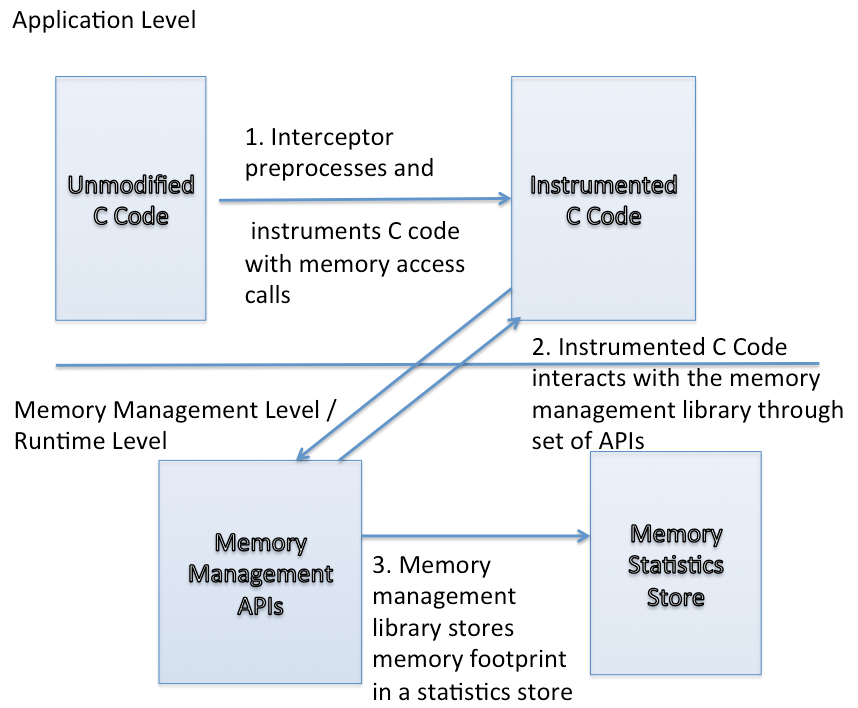
\includegraphics[scale=0.3]{./images/architecture.png}
\end{figure}

\paragraph{Interceptor: Transparent Instrumentation}
The interceptor uses preprocessing and code level instrumentation for injecting calls which enable the monitoring mechanism. In order to monitor object references, Tracer uses an interceptor which pre-processes standard C source code. The interceptor classifies literals into different classes of 8 different class types. {\emph{Identifiers}} allocated as dynamic objects are identified as {\emph{trace targets}}. The interceptor adds an {\emph{access}} function call ({\emph{mem\_access}}) following an access to each {\emph{trace target}}. This {\emph{mem\_access}} library call increments the object's hidden count variable by one. 
\paragraph{Header Tagged Objects}
Tracer implements a custom version of the standard malloc library function named "{\emph{hmalloc}}" (header memory allocator) which {\emph{transparently}} tags each target object with a header field. The header acts as a custom metadata store for the object. The design philosophy behind tagging objects with headers is to be able to support faster count updates. Our earlier design was plagued by heavy overheads involved in looking up each objects counter within a hash table. {\emph{Object headers}} provide a clean solution to this problem since the metadata is now tagged to each object in memory. {\emph{Hmalloc}} increases the amount of bytes requested by the size of an int, and uses the additional space allocated to store the object count. A pointer to the memory location immediately following these four bytes is then returned to the requesting application. These objects are then added to an object list that Tracer manages, which is a part of the memory statistics store (described below).
\paragraph{Memory Monitoring Interfaces}
We provide the following interface to the application developer for getting memory statistics:
\begin{enumerate}
\item {\emph{void * hmalloc (size\_t bytes)}} - Allocates "bytes" size object tagged with a header.
\item {\emph{void hfree}} - Frees objects tagged with headers.
\item {\emph{void mem\_access\_stat}} - Prints the access count of all the objects allocated by the current program.
\item{\emph{void mem\_access(void *memory\_location, int count)}} - Increases the access count of the object at the memory location (memory\_location) by the count. This function is used by the memory interceptor to monitor access counts at the object-level.
\item {\emph{int mem\_access\_count(void *object\_address)}} - Returns the current access count of the object (at memory location "object\_address").
\end{enumerate}

\section{Evaluation}
\label{sec:eval}
\paragraph{}
In order to measure the performance of Tracer, we performed a microbenchmark study using binary trees as an exemplar in-memory data structure. We performed four sets of tests for our microbenchmark study. We measured the overall time taken for the creation of nodes of a large binary tree. We also tested the overheads involved in the search, update and traversal operations. Our experiments were done on an Intel $i5$ virtual machine with a {\emph{2.5 GHz}} clock frequency. The DRAM size allocated to the virtual machine was {\emph{4GB}}. All the experimental results have been averaged over 10 different runs. 

\paragraph{}
We performed a comparative analysis and compared Tracer's overhead with the performance of an unmodified implementation in C (we call it the {\emph{vanilla C implementation}}). We also implemented a page protection mechanism, similar to the mechanism used in \cite{SSDAlloc} for tracking objects. Our primary objective behind the study was to measure the overall overhead of our memory monitoring mechanism and compare it with a page protection mechanism. The implementation of the page protection mechanism used a page buffer size of {\emph{25MB}} as suggested in \cite{SSDAlloc}.

\paragraph{Binary Tree Creation Tests}
The first test measured the overall overhead that Tracer has while monitoring the access to objects. We created trees containing 2500 to 25000 nodes. The experimental results indicate that Tracer invokes an overhead of around 20\% over the vanilla C implementation. The page protection mechanism has an overhead of three orders of magnitude (refer to Fig. \ref{fig:create}). The average time for creation of a binary tree with the vanilla C implementation is around 3.77 milliseconds, 4.5 milliseconds for Tracer and over 1 second for the page protection mechanism. One of the primary reasons for the poor performance of the page protection mechanism is the overheads involved in the eviction of an object from the page table and its subsequent insertion in the object table. This requires a system call (triggered due to access to a protected page), eviction of the page from the page buffer (overheads due to memory copy) and page materialization (requiring memory copy from the object table to the page buffer and a look up in the object table). 

\begin{figure}[!h]
\caption{Binary Tree Benchmark Results For Tree Creation}
\label{fig:create}
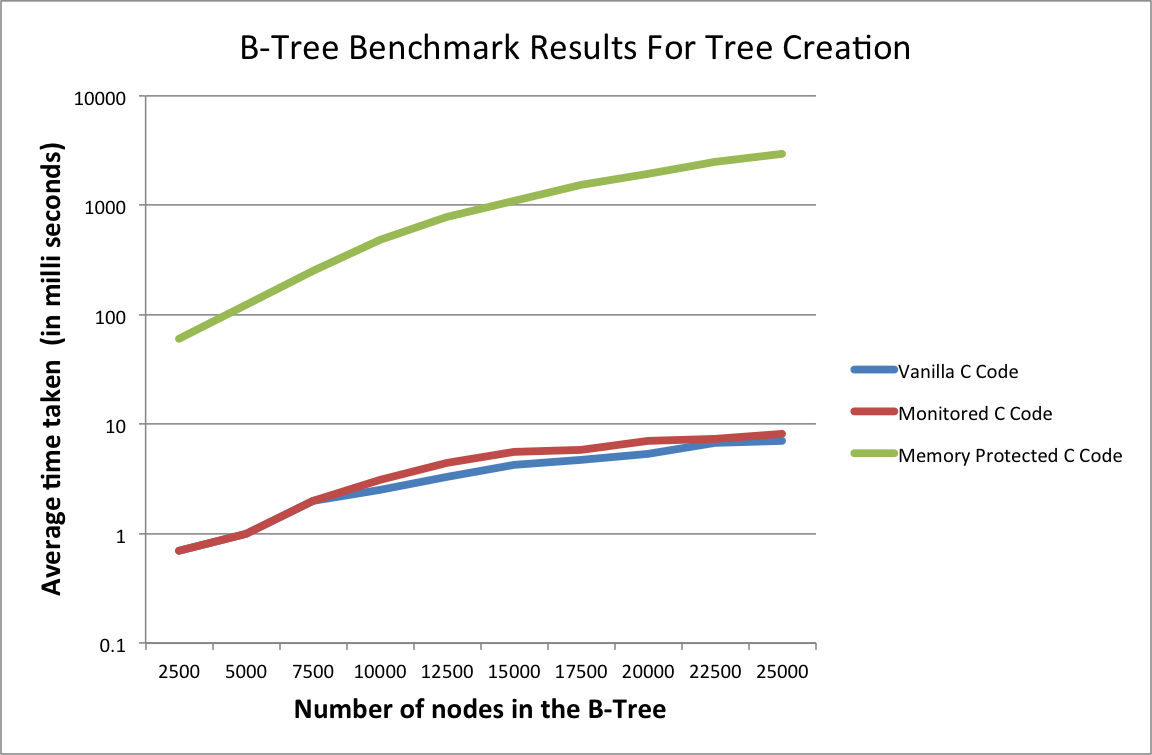
\includegraphics[scale=0.4]{./images/create.png}
\end{figure}
\begin{figure}[!h]
\caption{Binary Tree Benchmark Results For Read Workloads}
\label{fig:read}
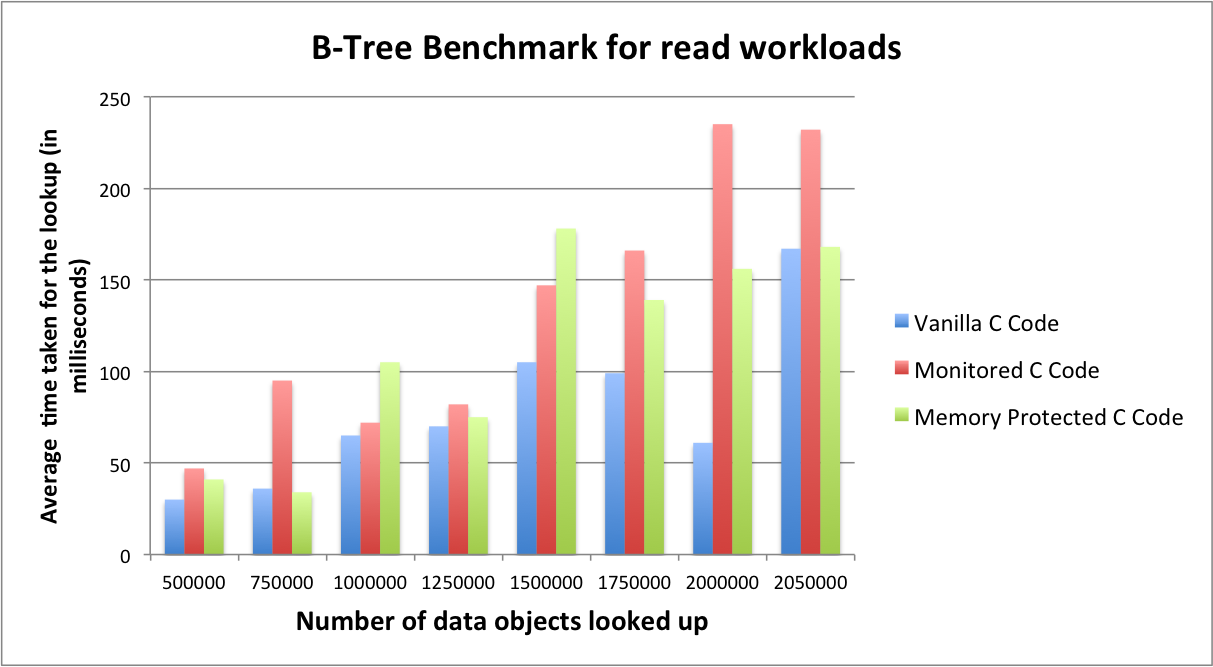
\includegraphics[scale=0.4]{./images/read.png}
\end{figure}
\begin{figure}[!h]
\caption{Binary Tree Benchmark Results For Update Workloads}
\label{fig:update}
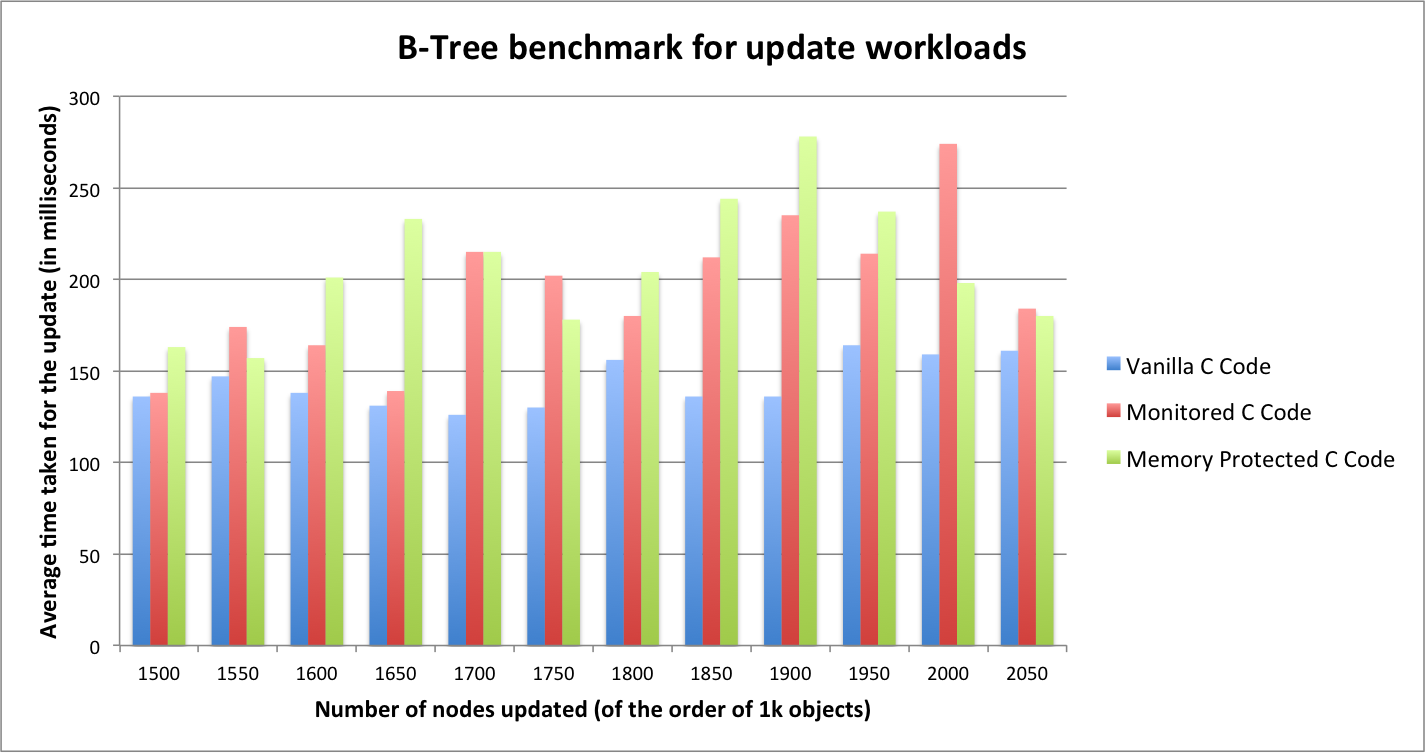
\includegraphics[scale=0.33]{./images/update.png}
\end{figure}
  

\paragraph{Binary Tree Read Tests}
The second set of tests measured the overall overhead incurred in reading a set of random objects from a Binary Tree of a fixed size (number of nodes in the binary tree was kept to 2500). For the read tests, we generated a random number of keys and search for them in a preconstructed binary tree. We varied the number of keys read from 500,000 to 2 million per experiment. Each data point is an average of 10 different experiments. Tracer has a reasonable overhead (of around $40\%$) over the vanilla C implementation, while the page protection mechanism has an overhead of $28\%$ (refer to Fig. \ref{fig:read}}). 
Tracer incurs slightly more overhead because it performs fine grained monitoring, whereas page protection mechanisms provide an approximation of the access pattern of the application. These overheads are reasonable considering the more precise information that Tracer provides the developer with.

\paragraph{Binary Tree Update Tests}
The third set of tests measured the overall overhead incurred for update intensive workloads. As in the read test, we generate a random set of key pairs. Each key pair has a source and a destination key. The source key is searched in the binary tree and its value is updated with the destination key's value. If the source key is not found in the binary tree then the update procedure returns. We varied the number of update operations from 1.5 million to 2.5 million for our tests. Tracer improves the performance of the update operations over the page protected mechanism by $6.28\%$. The overhead over the vanilla C implementation is around $35\%$. %(refer to Fig. \ref{fig:b-tree\_update.png}).
 These tests indicate that Tracer performs well in comparison to the page protection mechanism for update-heavy workloads. 

\paragraph{B-Tree Traversal Tests}
The fourth set of experiments explored the performance of tree traversals for the three different mechanisms. Tree traversals are generally observed heavily for range queries in databases. The page protected mechanism performs poorly for such workloads with over 2 orders of magnitude of overhead. 

\paragraph{}
The observation from the tree traversal and creation tests is that the page protection mechanisms perform poorly when a large number of nodes of the tree are touched. This could be explained because such an access pattern would result in a high "{\emph{object flux}}" between the page buffer and page table. The movement of an object between the page table and page buffer involves page eviction and page materialization which have high overheads. Tracer circumvents these overheads by its interception and tagged counter based approach. 

\section{Related Work}
\label{sec:related}
\paragraph{}
Memory tracing mechanisms such as Valgrind's memcheck \cite{nethercote2007valgrind}, gdb's ptrace \cite{gdb}, SSDAlloc's \cite{SSDAlloc} page protection mechanism rely on system call interfaces for  fine grained memory access. The overheads incurred due the reliance on system calls can downgrade the performance of the application. Kernel crossings result in interrupts to kernel, mode switches and data and instruction cache pollution. {\emph{Indirection}} mechanisms (such as those based on handles) have been previously used in HAC \cite{castro1997hac} and Mac memory management systems. Handle, based approaches trade off backward compatibility and provide finer monitoring of application data. We next describe systems based on memory protection mechanisms.

\paragraph{SSDAlloc's page protection mechanism}
SSDAlloc monitors fine grained access patterns through the use of an Object Per Page model, where each object is placed in its own page of virtual memory. SSDAlloc's DRAM is split into an object cache (which composes most of DRAM), and a Page Buffer that holds the set of materialized pages currently being used by the application (where each object is stored in its own physical page). SSDAlloc protects all virtual memory that it allocates, so any memory access for an unmaterialized page generates a page fault and is sent to SSDAlloc's interrupt handler. The handler would then pull the object from the object cache or the SSD, unprotect it and materialize it in the page buffer, and send it back to the application. This allows SSDAlloc to track memory accesses at an object level granularity as opposed to a page level granularity, since each virtual memory page access can be directly mapped to a single object access. Workloads that touch larger memory segments (such as tree creation, tree traversal) may not be fully resident within the page buffer. This could lead to heavy overheads due to interrupt call, object eviction from page buffer and page materialization.

\paragraph{Chameleon's memory tiering mechanism}
Chameleon improves on SSDAlloc's design by removing the need to split DRAM into a cache and page buffer entirely. Each object is still put into a single virtual page, but the virtual pages are partitioned into a set of object sized chunks, and the object is randomly placed into one of these chunks in the virtual page. Since these chunks can be mapped to a chunks in a physical page, a single physical page can store objects from multiple virtual pages. Chameleon requires memory object alignment at boundary offsets. This could lead to some memory wastage over standard memory allocation schemes. As with SSDAlloc the OPP model increases TLB pressure. Tracer does not make such assumptions for tracking object accesses.

\paragraph{Memory tracing systems}
Our design is inspired from {\emph{memlet}} based systems. {\emph{Memlets}} are small pieces of code which are injected into application code. These code sequences execute additional code for every memory access and monitor application access pattern at  a finer granularity. Memlets are generally weaved into into application code through {\emph{binary translation techniques, watchpoints, taint checking and data flow analysis}}.
Binary translation techniques modify code after the the application has been compiled to binary format. Binary translators {\cite{nethercote2007valgrind,bellard2005qemu}}convert programs to intermediate representation and then perform dynamic or static translation to improve the overall performance. Greathouse et al. \cite{greathouse2012case} describe a system for adding unlimited {\emph{watchpoints}} using hardware extensions (bitmap translation look aside buffer and a range cache) which can provide fine grained memory monitoring. Taint checking \cite{newsome2005dynamic, ho2006practical} and data flow analysis systems use additional taints per memory location and registers for registering accesses to them. Tracer "taints" memory structures with metadata (as headers) for monitoring accessing and updating access count information.

\paragraph{}

\section{Conclusions}
\label{sec:conclusion}



%% Bibliography
%\vspace{-1ex}
%\linespread{1.0}
%\setlength{\bibsep}{1pt}
%\footnotesize
\small
\bibliography{local}
\bibliographystyle{abbrvnat}

\end{document}

